\title{Průběžná hra TOČJ 2024: Hanza} 
\author{Petr}
\date{\today}

\documentclass[a4paper, 12pt, twoside]{article}
\usepackage[czech]{babel}
\usepackage{graphicx}
\usepackage{url}

\usepackage{marginnote}

\usepackage[top=1.5cm, bottom=2.0cm, outer=1.5cm, inner=3.5cm, heightrounded, marginparwidth=0cm, marginparsep=0cm]{geometry}
%\addtolength\oddsidemargin{1cm}
%\addtolength\evensidemargin{-1cm}

\usepackage{xcolor}
\usepackage{hyperref}
\usepackage[normalem]{ulem}
\usepackage{enumitem}
\usepackage{amsmath}
\usepackage{amsfonts}
\usepackage{float}
\usepackage{wrapfig}
\usepackage{multicol}

\DeclareSymbolFont{extraup}{U}{zavm}{m}{n}
\DeclareMathSymbol{\varheart}{\mathalpha}{extraup}{86}
\DeclareMathSymbol{\vardiamond}{\mathalpha}{extraup}{87}

\newcommand{\suits}{$\{\color{red}\varheart \color{black},\color{red} \vardiamond \color{black},\clubsuit , \spadesuit\}$}
\newcommand{\pozn}[1]{\marginpar{\textbf{Pozn}.: #1}}

\newcommand{\cheart}[1]{$#1\color{red}\varheart$}
\newcommand{\cdiamond}[1]{$#1\color{red}\vardiamond$}
\newcommand{\cclub}[1]{$#1\clubsuit$}
\newcommand{\cspade}[1]{$#1\spadesuit$}

\usepackage{fancyvrb}
\newcommand\userinput[1]{\textbf{#1}}
\usepackage{tgcursor}

\begin{document}
\newgeometry{left=2cm, right=2cm}
\maketitle

\begin{multicols}{2}
\tableofcontents
\end{multicols}

\restoregeometry
\newpage{}

\section{Úvod (hra v kostce)}

Družinky představují obchodníky.  S pomocí lodí (které průběžně staví a pojmenovávají) převáží zboží mezi hanzovními městy.  Každé 
město nabízí a poptává jiné typy zboží.
Ve hře pro zjednoduššení nejsou peníze, ale i tak budeme používat termíny jako \emph{koupit} či \emph{prodat}.  Při nakupování nic neplatíte a při
prodeji nic nekasírujete.

Družinky též vysílají své delegáty (konšely) do městských rad, kde tito společně vymýšlejí zákony, kterými se následně řídí obchod a stavba lodí v konkrétních
městech.

Hra je tahová, každý táborový den se odehraje jedno herní kolo\footnote{Změna v případě katastrofy či z jakéhokoli jiného důvodu je vyhrazena.}. 

\subsection{Cíl hry}

Cílem hry je prodat do měst co největší objem zboží.  Družinka získává body vždy, když město spotřebuje zboží družinkou dodané.  Vyhrává ta družinka, 
která má na konci hry nejvíce bodů.



\begin{wrapfigure}{r}{0.2\textwidth}
\centering
\includegraphics[width=0.2\textwidth]{figs/danzigG.png}
\caption{Svobodné město Danzig (dnešní Gdaňsk)}
\label{danzig}
\end{wrapfigure}

\section{Základní definice}

\subsection{Komodity}

Ve hře se vyskytují 4 obchodní komodity, z nichž každé náleží jedna barva z klasického balíčku na poker:

\begin{itemize}
    \item \cheart{} = pivo
    \item \cspade{} = sledi
    \item \cdiamond{} = látky
    \item \cclub{} = dřevo
\end{itemize}

\subsection{Náklad}

Náklad představuje nedělitelný objem zboží určený k obchodu.  Jeden náklad je reprezentován jednou kartou z balíčku na poker.

Náklad má dva parametry -- komoditu a velikost.  Pro číselné karty (2 až 10) je velikost číslo vytištěné na kartě.  Karta A má velikost 1,
karty J,Q,K mají velikost 5.

\subsection{Loď}

K obchodu s náklady slouží lodě.  Každá loď má unikátní jméno a patří konkrétní družince.  Lodě se pohybují po mapě mezi městy, ve kterých můžou kupovat a 
prodávat náklady.  Loď je na mapě reprezentována špendlíkem v barvě družinky, na který je navázaný papír se jménem lodi.

Ke každé lodi patří jeden list do sběratelského alba.  Do prvního políčka se vkládá lísteček se jménem 
lodi a datem dne, kdy byla loď postavena.\footnote{Na lísteček se jménem lodi je povoleno (nikoliv vyžadováno) nakreslit loď.  Nakreslená loď nemá žádnou herní funkci, ale bude to krásné.}
.  Do zbylých se vkládají náklady na loď
naložené.  Na loď lze najednou naložit maximálně 8 karet nákladů a \textbf{součet velikostí naložených nákladů nesmí přesáhnout 15}.

\begin{wrapfigure}{r}{0.5\textwidth}
\centering
\includegraphics[width=0.5\textwidth]{figs/kamzikG.jpg}
\caption{Příklad lodi}
\label{prlod}
\vspace{-50pt}
\end{wrapfigure}

V příkladu z obrázku \ref{prlod} jsou na \emph{Bledém kamzíkovi} naloženy dva náklady piva a jeden velký náklad dřeva.  Součet velikostí nákladů je 13 -- 
kdybychom chtěli, mohli bychom na loď přidat ještě jeden náklad o velikosti 2 nebo dva náklady o velikosti 1.

\subsection{Mapa}

Mapa, po které se pohybují lodě, obsahuje 14 políček.  12 z těchto políček představuje hanzovní města, 2 políčka
(šedé čtverce) představují neosídlené oblasti, kterými lze plout, ale nelze v nich obchodovat.

Mezi políčky jsou na mapě nakreslené spojnice, které udávají, kudy mohou lodě plout.

\subsection{Město}

Ve hře je 12 hanzovních měst.  Každé město má následující neměnné parametry:  jméno, umístění na mapě, komodita kterou město prodává a komodita
kterou město kupuje.  Město je na mapě reprezentováno osmiúhelníkem.

Například v městě Danzig (obrázek \ref{danzig}) prodávají pivo (\cheart{}) a kupují sledě (\cspade{}).

\subsubsection{Trh}
\label{trh}

Městský trh tvoří tři políčka v listu do sběratelského alba.  
Do políček se vkládají náklady.  Náklady vložené lícem vzhůru jsou v \emph{nabídce} města -- lze je v městě koupit.  
Naopak pokud do města náklad prodáme, vloží se do políčka lícem dolů -- do \emph{poptávky}.

\textbf{Každá družinka má v každém městě svůj vlastní, oddělený, trh.}  Tedy skutečnost, že družinka A v Danzigu něco koupila či prodala, nijak neovlivňuje
obchodní možnosti družinky B tamtéž.

Jak v nabídce města, tak v poptávce města mohou být najednou maximálně 3 karty nákladů.  Do nabídky v každém kole náklady přibývají, z poptávky naopak každé
kolo mizí, viz \ref{produkce_a_spotreba}.

\begin{figure}[h!]
\centering
\includegraphics[width=1\textwidth]{figs/trhv2G.png}
\vspace{-0.7cm}
\caption{Příklad trhu: pohled zepředu (vlevo) a zezadu (vpravo)}
\vspace{-0.2cm}
\label{trh_img}
\end{figure}

V situaci na obrázku \ref{trh_img} je právě možné v Danzigu zakoupit dva různé náklady piva, jeden o velikosti 8 a druhý o velikosti 5.

Kdybychom ale chtěli v Danzigu prodávat sledě, máme momentálně smůlu.  V poptávce už není žádné volné místo, musíme tedy s prodejem
počkat, až Danzigčtí pár ryb snědí.

\subsubsection{Obchodní zákon}

Ve městě může platit jeden obchodní zákon.  Obchodní zákon se vztahuje na některé lodě 
(v závislosti na jejich jméně) a různými způsoby je omezuje.
Obchodní zákon může být vytvořen či změněn na zasedání městské rady (viz \ref{mestska_rada}).

Příklad obchodního zákona:

\begin{itemize}
    \item Loď, která obsahuje slovo začínající písmenem K, zde nesmí kupovat náklady liché velikosti.
\end{itemize}

Takovýto zákon by se vztahoval na \emph{Bledého kamzíka}, ale třeba loď \emph{Bismarck} by jím nebyla dotčena.

Informace o tom, na které lodě se zákony kterých měst vztahují, budou k dispozici v průběžně aktualizované tabulce.  Tabulku vyplňuje vedení 
dle své interpretace zákonů.  Obsah tabulky je závazný, nadřazený zdravému rozumu a nelze se proti němu odvolat.

\subsubsection{Pravidla loděnice}

V každém městě vždy platí právě dvě pravidla loděnice.  Tato pravidla upřesňují, jak smí být pojmenovány 
lodě v tomto městě postavené (viz \ref{stavba_lodi}).
Na zasedání městské rady může být změněno jedno z pravidel loděnice.

Například, pokud v Danzigu platí následující dvě pravidla loděnice:

\begin{itemize}
    \item Loď zde postavená musí obsahovat název sudokopytníka.
    \item Loď zde postavená musí obsahovat přídavné jméno.
\end{itemize}

pak je v Danzigu možné postavit loď \emph{Bledý kamzík}.  Loď \emph{Drobný kůň} by zde však postavit nešla, neboť kůň je lichokopytník.

\subsection{Účetní kniha}

Každá družinka má svou účetní knihu (šanon), ve které jsou umístěny stránky do sběratelského alba reprezentující její lodě a její trhy v jednotlivých městech.

Účetní kniha je svatá a každý obchodník ji střeží jako oko v hlavě.  Se svými konkurenty se může o obsahu účetní knihy bavit, ale nesmí jim ji ukazovat.  

Je zakázáno nahlížet do cizích účetních knih.


\newpage

\section{Struktura herního kola}


\begin{wrapfigure}{r}{0.4\textwidth}
\vspace{-0.7cm}
\centering
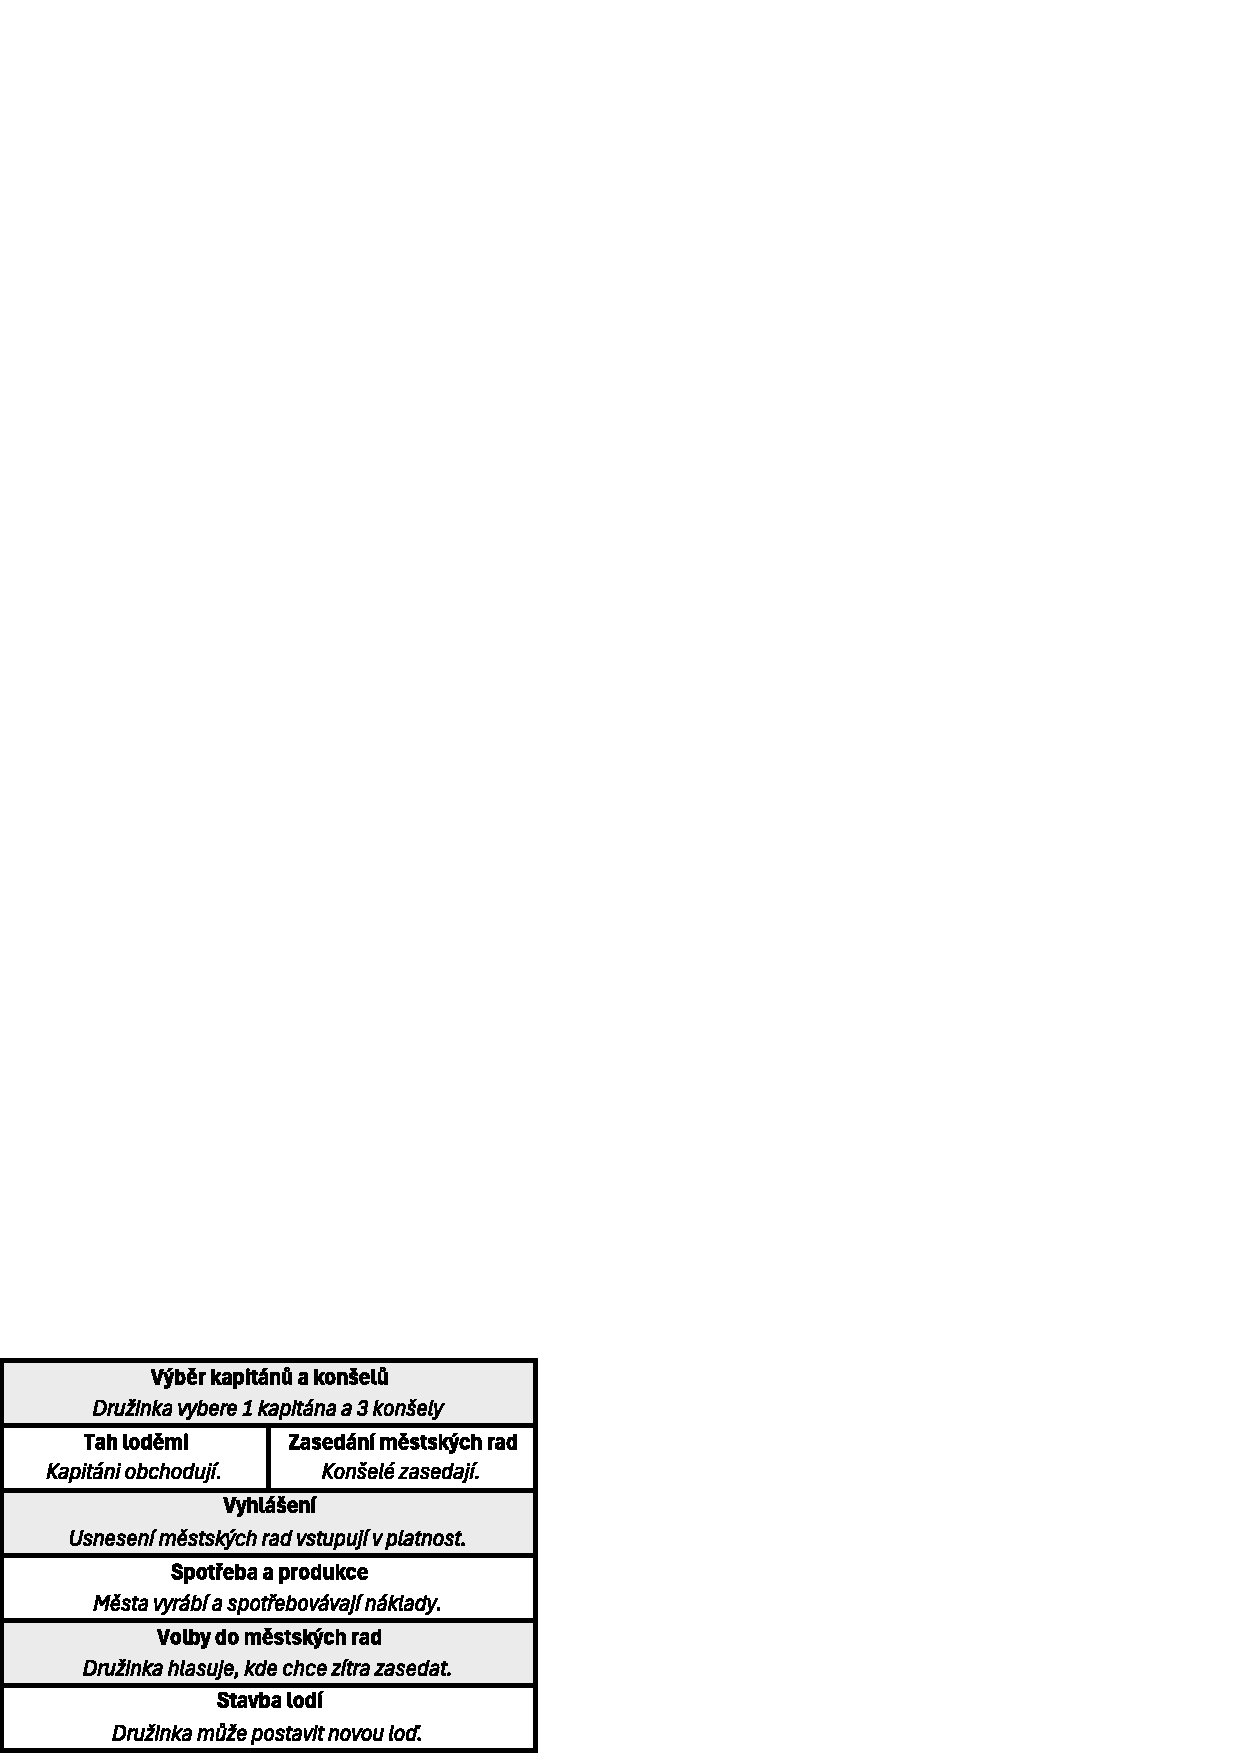
\includegraphics[width=0.4\textwidth]{figs/structaid.pdf}
\vspace{-0.7cm}
\caption{Fáze herního kola}
\label{structaid}
\end{wrapfigure}

Herní kolo se skládá z několika fází, které jsou detailně popsány v sekci \ref{faze}.

Po snídani probíhají současně fáze \textbf{tah loděmi} (\ref{tah_lodemi}) a \textbf{zasedání městských rad} (\ref{mestska_rada}).  
Družinka ze svého středu vybere jednoho \emph{kapitána}, který převezme účetní knihu a má na starosti tahy loděmi, a tři \emph{konšely}, kteří 
se odeberou na městské rady.
Tah loděmi probíhá v hangáru, zasedání ve stanech.  
Do konce těchto fází spolu nesmí kapitáni a konšelé nijak komunikovat. 
V tahu loděmi probíhá obchod s náklady, na zasedání městských rad se mezitím přijímají zákony a další rozhodutí.

Po dokončení těchto dvou fází následuje \textbf{vyhlášení} (\ref{vyhlaseni}), na kterém vybraní konšelé sdělí, co se odhlasovalo na zasedáních městských rad.  V této fázi
vstupují v platnost zákony na městských radách přijaté.

Další fáze je \textbf{produkce a spotřeba} (\ref{produkce_a_spotreba}).
V této fázi se v každém městě vyrobí jeden nový náklad.  Města se též pokusí spotřebovat náklady které jim byly prodány.  Průběh této fáze může být ovlivněn 
hlasováním na městských radách.

Po produkci a spotřebě následují \textbf{volby do městských rad} (\ref{volby}), kde družinky tajně vyjádří preference stran toho, ve kterých 
městech by chtěly zítra zasednout.  

Poslední fáze, \textbf{stavba lodí} (\ref{stavba_lodi}) probíhá individuálně během zbytku dne (když družinka vymyslí jakou loď chce postavit, odchytne
si vedení a loď postaví).


\section{Fáze herního kola}
\label{faze}

\subsection{Výběr kapitána a konšelů}

Družinka nejprve vybere ze svého středu jednoho \emph{kapitána}, který bude řešit plavbu a obchod družinkových lodí.  Výběr kapitána je libovolný, je povoleno opakovaně
vysílat toho samého kapitána.

Následně družinka vybere ze zbývajících členů tři \emph{konšely}, kteří zasednou na městských radách ve třech (předem vedením určených) městech.  
Konšelé se narozdíl od kapitána musí střídat: družinka musí přednostně do role konšela vybrat ty členy, kteří byli zatím vybráni nejméněkrát.  


\subsection{Tah loděmi}
\label{tah_lodemi}

Kapitán vyslaný družinkou postupně táhne všemi loděmi, které družinka momentálně na mapě má.  Pořadí lodí určuje kapitán.

Každá loď v této fázi vykoná 4 \emph{akce}.  Akce jsou trojího druhu: \emph{odpočinek}, \emph{plavba} a \emph{obchod}.

    \textbf{Loď nesmí jako svou první akci ve fázi vykonat obchod}.  Jinak může loď akce kombinovat libovolně.  Tah lodi může být třeba \emph{plavba--obchod--plavba--obchod}.

Pokud se na loď dle tabulky vztahují obchodní zákony, pak se těmito zákony musí kapitán při tazích příslušnou lodí řídit.

\subsubsection{Odpočinek}

Loď, která vykonává akci odpočinek, zůstává na svém místě a nedělá nic.

\subsubsection{Plavba}

Loď, která vykonává akci plavba, se posune na mapě ze svého políčka na některé sousedící políčko.  Sousedící políčka jsou spojena šipkou.

\subsubsection{Obchod}
\label{tah:obchod}

\textbf{Nelze vykonat jako první akci!}  Loď, která vykonává akci obchod, nejprve prodává, poté nakupuje náklady ve městě ve kterém se zrovna na mapě nachází\footnote{Pokud se loď nachází na políčku
neobydlené oblasti, nemůže vykonat akci obchod.}.

Loď může prodávat náklady té komodity, kterou město poptává.  Každý prodaný náklad se vyjme z lodi a vloží se do některého volného políčka v \emph{poptávce}
města (viz \ref{trh}).  Lze prodat pouze tolik karet nákladů, kolik je volných políček v poptávce.  

Loď může poté koupit libovolné náklady, které jsou v \emph{nabídce} města.  Při nákupu loď ale nesmí překročit svoji kapacitu -- maximálně může být na lodi
najednou 8 karet nákladů a \textbf{součet velikostí všech nákladů na lodi nesmí přesáhnout 15}.  (Náklady J,Q,K mají velikost 5, náklad A má velikost 1.)

\subsection{Zasedání městských rad}
\label{mestska_rada}

Každý den zasedají městské rady ve 4 městech.  Městská rada je tvořena třemi \emph{konšely}.  Každý konšel pochází z jiné družinky.  Každá družinka
právě v jednom z měst nemá zastoupení.

Plán zasedání městských rad (kdy zasedají rady ve kterých městech) bude vyvěšen na celý tábor dopředu.  
Která družinka bude zasedat kde se rozhodne den předem na základě fáze voleb do městských rad (viz \ref{volby}).

Městská rada zasedá ve stanu některého z konšelů.  Konšelé si na zasedání mohou přinést psané poznámky.  Konšelé v průběhu zasedání nekomunikují s nikým
mimo svou městskou radu\footnote{Komuniakce s vedením je povolená.} a lidé mimo městskou radu se nesnaží ji očumovat ani odposlouchávat.

Městská rada rozhoduje vždy prostou většinou.  Tedy pokud se na nějakém rozhodnutí shodnou alespoň dva ze tří konšelů, pak je toto rozhodnutí přijato.

\subsubsection{Agenda: Předpověď produkce}

Městská rada obdrží papír s informacemi o tom, jaké náklady budou v jejich městě dnes, zítra a pozítří vyrobeny ve fázi produkce a spotřeba.
Je povolené a žádoucí, aby si konšelé tuto předpověď poznamenali.

\subsubsection{Agenda: Volba hlasatele}
\label{volba_hlasatele}

Městská rada rozhodne, který z jejích členů se stane \emph{hlasatelem}.  Hlasatel má povinnost ve fázi vyhlášení přednést vše, na čem se rada
shodla.  (Předpověď produkce hlasatel nepřednáší.)

\subsubsection{Agenda: Usnesení o zvýšení produkce}
\label{agenda_produkce}

Městská rada se může shodnout, že podpoří produkci nákladů ve svém městě.  Pokud tak učiní, pak se v jejich městě dnes ve fázi produkce a spotřeba navíc vyrobí
jeden náklad o velikosti 5.

Tato bonusová produkce proběhne před běžnou produkcí a týká se všech družinek (i té, která ve městě nezasedala).

\subsubsection{Agenda: Usnesení o zvýšení spotřeby}
\label{agenda_spotreba}

Městská rada se může shodnout, že podpoří spotřebu nákladů ve svém městě.  Pokud tak učiní, pak se jejich město dnes ve fázi produkce a spotřeba pokusí 
spotřebovat navíc jeden náklad o velikosti menší než 5 (tedy A,2,3,4).  Město při bonusové spotřebě vybere největší náklad splňující tuto podmínku.

Náklad spotřebovaný v bonusové spotřebě přináší družince oproti běžné spotřebě 2 body navíc.  (Tedy např. při spotřebování nákladu velikosti 4 získá družinka 6 bodů).

Tato bonusová spotřeba proběhne před běžnou spotřebou a týká se všech družinek (i té, která ve městě nezasedala).

\subsubsection{Agenda: Změna pravidla loděnice}

Městská rada obdrží obě momentálně platná pravidla loděnice svého města.  Rada se může shodnout na tom, že jedno z těchto pravidel zruší a nahradí ho jiným.

Pravidlo loděnice musí být jednoznačně vyhodnotitelné a podléhá vetu starosty (viz \ref{veto}).

Městská rada nemůže zrušit obě pravidla loděnice najednou, aspoň jedno z původních zůstane v platnosti.

\subsubsection{Agenda: Novela obchodního zákona}

Městská rada se může shodnout, že ve svém městě vytvoří nový obchodní zákon.  Pokud již v jejich městě nějaký obchodní zákon platil, pak bude tento novým
zákonem nahrazen.

Obchodní zákon se skládá ze dvou částí -- \emph{zacílení} a \emph{efekt}.  Zacílení určuje, kterých lodí se zákon bude týkat, efekt popisuje postih, který
bude zákonem na lodě uvalen.  Městská rada stanovuje pouze zacílení zákona, efekt se následně vylosuje ve fázi vyhlášení (viz \ref{vyhlaseni}).

Zacílení musí splňovat následující podmínky:

\begin{enumerate}
    \item Zacílení je jednoznačně a snadno vyhodnotitelné.
    \item Zacílení bere v potaz pouze název lodi.
    \item Zacílení nemá formu seznamu názvů lodí nebo slov.
\end{enumerate}

Zacílení podléhá vetu starosty (viz \ref{veto}). 

\subsubsection{Starostovo veto}

\label{veto}

Poté, co městská rada odhlasuje nové zacílení obchodního zákona nebo nové pravidlo loděnice, musí jej předložit starostovi (definovanému členovi vedení), kterého
si za tím účelem přivolá.

Pokud starosta výplod městské rady schválí, příslušný bod agendy je tím vyřešen a městská rada nové zacílení či pravidlo loděnice napíše čitelně na papír o velikosti 2x10 cm.

Starosta může pravidlo/zacílení též bez udání důvodu vetovat.  V takovém případě zůstává bod agendy otevřen a městská rada se může pokusit najít shodu na
jiném řešení.  V případě že ji najde, opět si přivolá starostu.  Je zakázáno volat starostu znovu k pravidlu/zacílení ve stejném znění, jaké již jednou vetoval.


\subsection{Vyhlášení}
\label{vyhlaseni}

Hlasatelé zvolení na zasedání městských rad (viz \ref{volba_hlasatele}) postupně v přítomnosti zástupců všech družinek pravdivě přednesou, na čem se 
jejich městské rady shodly.  Konkrétně vyhlásí:  zda rada přijala usnesení o zvýšení produkce, zda přijala usnesení o zvýšení spotřeby, 
zda zavedla nové pravidlo loděnice (pokud ano, přečte obě platná pravidla) a zda novelizovala obchodní zákon.

Pokud se městská rada shodla na novele obchodního zákona, pak si hlasatel vylosuje efekt, který bude k novému obchodnímu zákonu přiřazen a výsledný zákon
přednese.

Vyhlášením vstupují veškeré změny v platnost.

\subsection{Produkce a spotřeba}
\label{produkce_a_spotreba}

Vedení si na začátku fáze od družinek vybere jejich účetní knihy, aby v nich mohlo provést produkci a spotřebu.

Fáze probíhá podle stejného algoritmu pro všechny družinky.


\subsubsection{Běžná produkce}

V každém městě je vyprodukován jeden náklad a umístěn do jeho nabídky.  Pokud v nabídce města není žádné volné políčko, pak vyprodukovaný náklad nahradí
\emph{největší} náklad v nabídce.

Komodita vyprodukovaného nákladu vždy odpovídá komoditě, kterou město nabízí.  Velikost vyprodukovaného nákladu se určí podle neveřejné předem vylosované
posloupnosti.  Karty do posloupnosti jsou losovány pro všech 12 měst po jednotlivých dnech z pokerových balíčků (bez karet J,Q,K) tak, že nový balíček
je načnut až ve chvíli, kdy je předchozí balíček vyčerpán.  (Pro detaily viz sekce \ref{nerd}).

\subsubsection{Bonusová produkce}

Pokud v městě dnes zasedala městská rada a schválila usnesení o zvýšení produkce, pak v městě proběhne \textbf{před} běžnou produkcí bonusová produkce.

Bonusová produkce se řídí stejnými pravidly jako běžná produkce s tím rozdílem, že vyprodukovaný náklad je vždy jedna z karet J, Q, K.

\subsubsection{Běžná spotřeba}

Každé město se pokusí spotřebovat největší náklad, který se nachází v jeho poptávce.  Družinka za spotřebovaný náklad získá počet bodů rovný velikosti
spotřebovaného nákladu.  Počty bodů jsou neveřejné (vedení sdělí pouze družince samotné).

\subsubsection{Bonusová spotřeba}

Pokud v městě dnes zasedala městská rada a schválila usnesení o zvýšení spotřeby, pak v městě proběhne \textbf{před} běžnou spotřebou bonusová spotřeba.

Město se v bonusové spotřebě pokusí spotřebovat největší náklad z poptávky, \textbf{který má velikost menší než 5}.  Pokud město nemá v poptávce
žádný náklad menší než 5, pak v bonusové spotřebě nic nespotřebuje.

Za náklad spotřebovaný v bonusové spotřebě družinka získá počet bodů o dva vyšší než je velikost nákladu.


\subsection{Volby do městských rad}
\label{volby}

Každá družinka odevzdá preferenční hlasovací lístek, na kterém seřadí města, ve kterých zítra zasednou městské rady, od 1 do 4.  1 znamená že 
zde rozhodně chtějí zasedat, 4 znamená že zde chtějí zasedat nejméně.

Vedení seřadí družinky podle momentálního počtu bodů\footnote{V případě plichty rozhodne los.} a počínaje poslední družinkou se pokusí co nejlépe vyhovět jejich přáním.

Tedy: družince která je poslední bude vyhověno a zasedne ve všech městech krom toho které označila jako 4.  Poté se vedení pokusí vyhovět předposlední družince
(pokud předposlední označila čtyřkou jiné město než poslední, pak předposlední bude vyhověno, pokud označila stejné, pak předposlední nebude zasedat ve městě
které označila jako 3.), atd.

Pro detaily viz sekce \ref{nerd}.

\subsection{Stavba lodí}
\label{stavba_lodi}

Tato fáze probíhá asynchroně až do večera podle principu kdo dřív příjde, ten dřív mele.  Každá družinka smí každý den postavit maximálně jednu loď.
Má-li družinka ve hře méně než 5 lodí, pak je stavba nové lodi povinná.

Družinka smí mít najednou ve hře maximálně 5 lodí.  Má-li jich už ve hře 5, může stále novou loď postavit, ale před samotnou stavbou musí jinou loď
\emph{odepsat} (viz \ref{odpis}).


\subsubsection{Stavba}

Družinka si vybere, ve kterém městě\footnote{V neobydlených oblastech loď postavit nelze.} chce loď postavit.  Následně příjde za vedením a sdělí mu název lodi, kterou by chtěla postavit.  Pojmenování lodi 
se řídí následujícími pravidly:

\begin{enumerate}
    \item Jméno nově postavené lodi není shodné se jménem žádné lodi, která byla někdy ve hře.
    \item Jméno nově postavené lodi nesdílí slovo se jménem žádné lodi, která je momentálně ve hře.
    \item Jméno lodi obsahuje slovo v prvním pádě.
    \item Jméno lodi obsahuje maximálně 5 slov.
    \item Jméno lodi splňuje obě pravidla loděnice města, ve kterém družinka loď staví.
\end{enumerate}

Pokud vedení vyhodnotí, že loď pravidla splňuje, loď je postavena, družinka ji umístí na mapu do vybraného města a v účetní knize si založí stránku pro 
loď (vloží do prvního slotu stránky do sběratelksého alba jmenovku lodi s dnešním datem).

Pro účely pravidla č. 2 výše uvažujeme, že změnou pádu, osoby, čísla, nebo stupňováním přídavného jména nevzniká nové slovo.

\subsubsection{Odpis staré lodi}
\label{odpis}

Pokud chce družinka postavit novou loď, ale již má ve hře 5 lodí, pak musí nejprve jednu loď odepsat.  \textbf{Není povoleno odepsat svou nejmladší loď}, 
je nutno odepsat jednu ze 4 starších.

Pokud družinka ke stavbě nové lodi vybere město, ve kterém se nacházela odepisovaná loď, pak náklady, které byly naložené na odepisované lodi, přechází
na novou loď.  Pokud družinka staví novou loď jinde, pak jsou náklady z odepsané lodi ztraceny (družinka odevzdá vedení
bez bodové kompenzace) a nová loď začíná prázdná.

Jméno odepsané lodi se poznamená veřejně do síně slávy (za účelem ověřování pravidla č. 1 pro stavbu lodí).

Pro účely pravidla č. 2 pro stavbu lodí uvažujeme, že odepisovaná loď již není ve hře.  Tedy je např. možné odepsat loď \emph{Krásná Praha} a ihned postavit \emph{Krásnější Brno}.

\section{Začátek a konec hry}

\subsection{Počáteční setup}

Na začátku hry je v nabídce každého města jeden náklad a poptávka všech měst je prázdná.

Ve městech na začátku hry neplatí žádné obchodní zákony.  Prvotní pravidla loděnic určuje vedení.

Před začátkem hry vedení určí náhodné pořadí družinek.  Následně proběhne jedna fáze voleb do městských rad, kde se místo počtu bodů k určení priority využije
toto náhodné pořadí.  

Po volbách do městských rad postaví všechny družinky dvě lodě.  Stavba lodí proběhne po jedné v obráceném pořadí než v jakém byly družinky prioritizovány ve volbách.



\subsection{Poslední den}

Poslední herní den skončí fází produkce a spotřeba, následující fáze se vynechají.

Veškeré náklady, které na konci hry zůstanou v poptávkách měst, se spotřebují (družinky získají body stejně, jako kdyby byly náklady spotřebovány při 
běžné spotřebě).

Náklady, které na konci hry zůstanou v nabídkách měst a naložené na lodích, jsou ztraceny bez bodové kompenzace.
\newpage{}
\section{Algoritmy pro nerdy}

\label{nerd}

Doplňková sekce pro fajnšmekry, kterým nestačilo vysvětlení některých herních mechanismů lidskou řečí.  Pokud ti stačilo, nemusíš ji číst.

\subsection{Losování sekvence produkce}

Rozdělme hanzovní města na 4 skupiny po třech podle komodity kterou produkují.  Nechť $P^{k}_{i}(d)$ značí velikost nákladu vyprodukovaného v i-tém městě k-té
skupiny v herním dni d.  Produkce pro $d=0$ představuje počáteční setup nákladů ve městech.  Uvažujme balíček karet na poker ze kterého byly vyjmuty karty J,Q,K všech barev, tedy 4x\{A,2,3,4,5,6,7,8,9,10\}.  Dále nechť zápis
$karta(k)$ značí náhodný výběr jedné karty z aktivního balíčku v barvě odpovídající komoditě k-té skupiny.

Postup losování tajné sekvence produkce popisuje následující pseudokód: \\
\null \\
\noindent\makebox[\textwidth][c]{
\fbox{\begin{minipage}{25em}
  \null \quad\emph{Načni nový balíček.}
\\  \null\quad  \textbf{pro} D v \{0, 1, 2, ... 11\}:
\\ \null\quad\quad \textbf{pro} I v \{0,1,2\}:
\\  \null\quad\quad\quad \textbf{pokud} je balíček prázdný:
\\  \null\quad\quad\quad\quad\emph{Načni nový balíček.}
\\  \null\quad\quad\quad \textbf{pro} K v \{0,1,2,3\}:
\\  \null\quad\quad\quad\quad $P^{K}_{I}(D) \gets karta(K)$\\
\null
\end{minipage}
}
}

\subsection{Vyhodnocení voleb do městských rad}

Problém rozhodnutí, ve kterých třech městech družinka zasedne, je ekvivalentní problému rozhodutí, ve kterém jednom městě nezasedne.

Přiřaďme družinkám identifikátory $\alpha$, $\beta$, $\gamma$, $\delta$ tak, aby toto pořadí odpovídalo momentálním počtům bodů družinek (tj. družinka $\alpha$ má 
nejvíc bodů, družinka $\delta$ nejmíň.)  Přiřaďme městům, ve kterých dnes zasedají rady, identifikátory A,B,C,D.  
Nechť zápis $hlas(d,i)$, kde $d$ je identifikátor družinky a $i$ je číslo od 1 do 4, označuje město které družinka d na svém hlasovacím lístku umístila na i-tou pozici.
Dále nechť zápis $absence(M)$ značí družinku, která v městě M nezasedne.  Vyhodnocení voleb proběhne podle následujícího algorimtu:

\noindent\makebox[\textwidth][c]{
\fbox{\begin{minipage}{25em}

  \null \quad   \textbf{pro} M v \{A,B,C,D\}: \\
  \null \quad   \quad $absence(M) \gets 0$ \\
  \null \quad   \textbf{pro} D v $\{\delta, \gamma, \beta, \alpha\}$: \\
  \null \quad \quad $i \gets 4$ \\
  \null \quad \quad \textbf{dokud} $absence(hlas(D, i)) \neq 0$: \\ 
  \null \quad \quad \quad $i \gets i - 1$ \\
  \null \quad \quad $absence(hlas(D, i)) \gets D$ \\
  \null
\end{minipage}
}
}

Družinka $\delta$ tedy vždy bude absentovat ve městě, které umístila na 4. pozici.  






\end{document}